\chapter{Алгоритмическое обеспечение и адаптация алгоритмов}

В этой главе рассматривается задача адаптации существующих алгоритмов, используемых в различных системах АДТ для повышения производительности процесса поиска логических выводов, \app{а также разработка других специализированных алгоритмов}. Задача этой главы -- реализовать полезные свойства ПО--исчислений при помощи известных мощных алгоритмов поддержки различных этапов построения логических выводов. В качестве таких алгоритмов выбраны: разделение данных (data sharing) \cite{Che2, Ryazanov2003}; индексирование данных (term indexing) \cite{HARIndex, TermIndexingBook,pathindex}; параллельные стратегии \cite{PSETHEO}; стратегия ограниченных ресурсов \cite{Ryazanov2003}; кэширование данных; расширена стратегия k-опровержения \cite{ICDS2000, dissChe} до стратегии k,m-ограничения; для эффективной работы с предикатом равенства использованы результаты теории переписывания термов \cite{Nipkow}. Предложен ряд стратегий работы с неограниченными переменными. Разработана структура данных дерево состояний вывода, позволяющая реализовать одновременно некоторые из перечисленных стратегий. 

В результате адаптации получены следующие результаты: значительное экономие памяти, влекущее за собой экономию вычислительных ресурсов за счёт того что предотвращается излишнее копирование термов и целых подформул; рост производительности с использованием параллельных стратегий (при условии применимости этих стратегий); сокращение пространства поиска за счет стратегий k,m-ограничения, ограничивающее разростание формулы за счёт дизъюнктивного ветвления, и неограниченных переменных (позволяющих не перебирать эрбранов универсум.  

%==========================================================
\section{Предпосылки разрабатываемых алгоритмов}

Для того что бы алгоритмы адекватно использовали возможности ПО--формализма необходимо выявить его совместимые полезные свойства, а также свойства, не совместимые с адаптируемыми алгоритмами.  Полезные свойства, которые обеспечены алгоритмически в рамках данной диссертации представлены во введении.

%--------------------ПРОБЛЕМЫ------------------------------------
\subsection{Проблемы формализма ПО-формул}
Укажем на некоторые свойства ПО-формализма, сказывающиеся на \rem{производительности процесса поиска ЛВ и ...}{Как оно сказывается?} в частичном разрешении которых он нуждается.

\begin{enumerate}

\item Поиск ответов на вопросы с открытыми переменными требует выбора   подставляемого терма для данной переменной из эрбранова универсума,   который, в общем случае, т.е. при наличии функциональных символов, является бесконечным множеством (счетным множеством). Какой именно терм необходимо выбрать --- изначально неизвестно.

Сделаем несколько замечаний. Во-первых, при решении прикладных задач, переменные связанные квантором всеобщности ограничиваются типовым условием, а значит появление открытых переменных в данном случае следует рассматривать как некую аномалию в следствии неверной формализации задачи. Это значит, что решение данной проблемы лежит вне прикладной области, и необходимо для решения общематематических теорем, например, из библиотеки TPTP.  Во-вторых, есть соблазн уйти от функциональных символов (как это скромно сделано в \cite{ICDS2000}), но наличие функциональных символов есть основа сложных задач. В-третьих, в \cite{ICDS2000} предложена идея стратегии решения данной проблемы --- стратегия отсроченного присваивания (СОП), заключающаяся в том что изначально для открытой переменной выбирается неопределенный эрбранов элемент, а позднее он постепенно доопределяется. Подробное описание стратегии и её реализация представлены в главе 3. Данная стратегия конфликтует с другими стратегиями. Однако анализ решаемых задач показывает что в \app{указанных} прикладных задачах нет нужды использовать СОП, т.к. в их формальном представлении нет открытых переменных. В общих же задачах сложнее найти какие-то особенности, которые применяются другими стратегиями, а значит конфликт частично разрешается просто разграничением областей применения \rem{системы}{Или же алгоритма   поиска подстановки для НЭЭ?}.

\item Язык ПО-формул в \cite{ICDS2000} характеризуется как <<достаточно   однородной, но в то же время хорошо структурированный>>, а \app{его исчисления}  <<хорошо усваивают эвристики>>, т.е. базовая стратегия исчисления достатосно легко настраивается под конкретную задачу. Стоит заметить, что однородность ПО-формул \rem{хуже}{В каком смысле? По отношению к чему? критерий.} чем, например, однородность дизъюнктов, в силу \rem{разнородных}{большего разнообразия?} сущностей в структуре формулы: база, вопросы, консеквенты вопросов. Разрешение \rem{данного вопроса}{Какого? Я не понял.} требует применения специальных методов доступа к \rem{данным неоднородным частям}{неоднородным частям ПО--формулы?}.

\item Хотя изначально представление формулы ИП в языке ПО--формул более компактно чем КНФ, применение правила вывода в ходе построения ЛВ при наличии дизъюнктивного ветвления, в общем случае, приводит к б\'{}ольшему усложнению структуры формулы, чем при применении правила вывода в методе резолюций. Таким образом, через некоторое количество шагов вывода размер ПО--формулы может оказаться в разы больше чем размер соответствующей КНФ. Но эта проблема практически полностью устранима технически, а именно описанными далее методами разделения общей оперативной памяти данных, а также ограничивающей стратегией, которую пользователь выбирает сам.
\end{enumerate}


%---------------------------
\subsection{Постановка задачи}
Поскольку в данной работе рассматривается первопорядковый язык ПО--формул, некоторые из структур данных и алгоритмов имеют сходства с уже существующими системам АДТ первого порядка. Это касается структуры термов и представления подстановок. Кроме того, существуют общетехнические методы \app{решения конкретных технических задач}, не зависящие от реализуемого формализма, например параллельные схемы алгоритмов, экономия потребляемой памяти, индексирование данных. Таким образом, в работе осуществлена адаптация некоторых существующих алгоритмов, используемых в современных эффективных системах АДТ. Адаптация предполагает, во-первых, учет особенностей ПО--формализма, как совместимых с данными алгоритмами, так и проблемных; во-вторых, \app{реализована} задача обеспечения совместимости адаптируемых алгоритмов, поскольку некоторые из них конфликтуют друг с другом при прямой независимой реализации.



%===============================================================
%---------------------------------------------------------------
%-----------------------АЛГОРИТМЫ---------------------------
\section{Алгоритмы и структуры данных}

%===================базовые структуры данных========================
\subsection{Общие структуры данных}

\app{Это реализация или алгоритмы, причем тут типы? Алгоритм+Стр. данных = Программа (Вирт))}

\paragraph{Тегирование структур данных.} 
Для различения данных используются слдеюущие теги: ATOM (атомарный символ), FUNCTION (функциональный символ), CONSTANT (константный символ), AVARIABLE (универсальная переменная), EVARIABLE (экзистенциальная переменная), UHE (Неопределённый Эрбрановский Элемент), INTEGER (целочисленный символ), FLOAT (нецелочисленный символ), STRING (строковый символ). Данные значения теговых полей структур определяются перечислением:

{\tt enum SymbolType \{CONSTANT, EVARIABLE, AVARIABLE, FUNCTION, ATOM, INTEGER, FLOAT, STRING, UHE\};}

\paragraph{Символ (Symbol).} 
Символ -- это идентификатор, используемый при построении терма. Структура \texttt{Symbol} содержит: 
\begin{enumerate}
\item Строковое представление символа. Необходимо для удобного (читаемого) вывода формулы на экран.
\item Тегирование символа, одним из перечисленных выше тегов. 
\item Арность. Числовое значение указывающие на количество аргументов. Для констант, переменных, числовых символов и строк, значение равно нулю.
\end{enumerate}

Символ идентифицируется его адресом в оперативной памяти ЭВМ.

\paragraph{Обобщённый терм (GTerm).} 
Названия для структуры взято из \cite{NNN}. Данная рекурсивная структура данных используется как для представления термов, так и атомов, в виде деревьев. 

Разные термы требуют соответствующих способов работы с ними. Например, вместо универсальной переменной можно подставить другой терм, тем самым конкретизировав её, вывод на экран конкретизированной и неконкретизированной переменной отличается; работа со структурами представляющими функции, требует учёта наличия аргументов; вместо НЭЭ не может быть подставлена универсальная переменная и т.д. Поэтому способ работы с термом зависит от символа, лежащего в корне дерева представляющиего данный терм. Символ несёт необходимую информацию, в том числе тег. Исходя из символа, в терме выделяется необходимое количество памяти под аргументы или возможные подставноки.  

Терм представляется классической рекурсивной древовидной структурой каждый узел которой содержит символ \app{\texttt{GTerm}} верхнего уровня и массив ссылок-аргументов. Универсальная переменная (AVARIABLE) и неопределённый эрбрановский элемент (UHE) не содержат никаких дочерних узлов, но используют единственный элемент одноэлементного массива ссылок-аргументов как ссылку на терм, который подставляется вместо термов AVARIABLE и UHE, таким образом производится конкретизация. Если эта ссылка указывает на NULL, значит соответствующая переменная ( или НЭЭ) конкретизированна некоторым термом. В противном случае переменная (или НЭЭ) является свободной для подстановки. Если переменная (или НЭЭ) конкретизированы, то терм представляющий переменную в данный момент представляет конкретизирующий терм. При этом глубина конкретизации может быть сколько угодно большой, например при такой подстановке ${\theta}_d = \{x \rightarrow h_1, h_1 \rightarrow h_2, h_2 \rightarrow e \}$, где $x$ --- универсальная переменная, $h_1, h_2$ это НЭЭ, а $e$ --- константа. После применения ${\theta}_d$, переменная $x$ фактически конкретизирована до константы $e$, и дальнейшая работа с термом $x$ производится как с константой $e$ (в том числе вывод на экран). Для корректной работы с конкретизациям реализован метод {\tt GTerm getValue()}, который возвращает самую глубокую конкретизацию данного терма. Если заданный терм $t$ не является переменной/НЭЭ или в противном случае если переменная/НЭЭ не кокретизирована, то значение getValue() совпадает со ссылкой на $t$. Иначе возвращается ссылка на самый глубокий терм, которым конкретизированна переменная/НЭЭ. Описанная выше работа с термами необходима для что бы корректно и эффективно откатывать подстановки, для этого необходимо сохранять информацию о том какая переменная/НЭЭ была конкретизирована, и чем. Для того что бы распознать конкретизацию достаточно проверить первый аргумент массива аргументов на NULL, а для того что бы откатить подстановку, значению аргумента присваивается NULL. 

\paragraph{Подстановка.} Подстановка есть список связей (binding) вида $X \rightarrow t$. В структуре Binding для $X$ и $t$ даны имена left и right соответственно. Определены следующие методы:

apply() --- применить подставноку. В каждой связи терм left связывается с термом right, т.е. аргумент left ссылается на right. 

reset() --- сброс подстановки. Аргумент left являющийся переменной приводится в состояние NULL, а left являющийся НЭЭ не сбрасиывается. Применяется непосредственно после шага вывода, для того что бы освободить переменные для дальнейшего использования, но при этом оставить НЭЭ связанными.

fullReset() --- сброс всей подстановки, включая НЭЭ. Применяется на этапе неудачной унификации, что бы вернуть все НЭЭ в прежнее состояни


%----------------------ЧАНК-------------------------------
\paragraph{Чанк} --- это односвязный список элементов типа {\tt T}, в котором выделен его первый ({\tt first}) и последний ({\tt last}) элемент. Чанк называется пустым, если он не содержит элементов, при этом first и last принимают значения NULL. Будем говорить что чанк $C_1$ связан с чанком $C_2$ слева, если узел last чанка $C_1$ ссылается на узел first чанка $C_2$, при этом $C_2$ связан с $C_1$ справа. Для связи чанков определена процедура связывания {\tt void link(Chunk!(T) c)}, которая связывает слева текущий чанк и чанк {\tt c}. Если чанки не пусты, то связывание производится согласно опредеению. Если один из чанков пуст, то при связывании его элементам first и last присваивается значение того элемента с которым он связывается. Отметим, что несколько чанков могут быть одновременно связанаы с другим чанком с одной его стороны. Таким образом процедурой связывания можно построить дерево чанков, растущее от листьев.

На рисунке \ref{fig:chank1} представлен пример структуры, образованной чанками.

\begin{figure}[h]
	%\vspace{0.5cm}
	\centering
	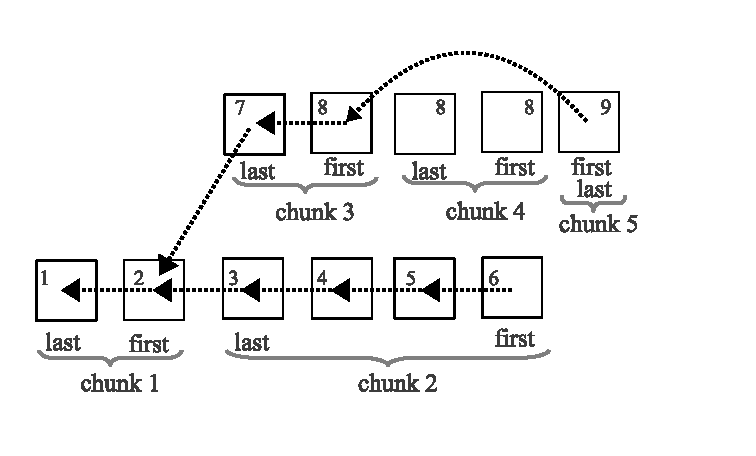
\includegraphics[width=0.6\linewidth]{pics/ChunkFull.eps}
	\caption{Чанки}
	\label{fig:chank1}
\end{figure}

Здесь изображено 5 чанков. Связаны слева следующие чанки: 5 и 4, 4 и 3, 3 и 1, 2 и 1. Чанк 4 являтся пустым. first  и last это первый и последний узлы чанков. Числа обозначают идентификатор узла. Отсюда видно что пустой чанк дублирует узел first. связанного слева с ним чанка.

Поясним смысл данной структуры. В отдельный чанк заносится информация о состоянии текущего шага логического вывода, поскольку информация разнородна, то для каждого конкретного случая тип {\tt T} конкретизируется. Связанные чанки образуют совокупность информации о шагах логического вывода. 




%=================== ДЕРЕВО СОСТОЯНИЙ ВЫВОДА =======================
\subsection{Дерево состояний вывода}
Одним из основополагающих средств реализации поиска ЛВ в разработанной системе АДТ является дерево состояний вывода (ДСВ), которое строится в основном при помощи структур данных, базированных на чанках. В структурах ДСВ, с одной стороны хранится вся совокупность шагов вывода, по которой можно распознать какие действия были произведены на каком шаге, с другой стороны ДСВ представляет текущю опровергаемую формулу. Основная задача ДСВ заключается в том, чтобы строго зафиксировать все события, произошедшие на каждом шаге логического вывода. \app{Примером фиксируемого события является факт применения некоторой подстановки к в некоторой базовой подформуле к некоторому вопросу}. Такая фиксация событий позволяет:
\begin{enumerate}
 \item Использовать больше информации о выполненных действиях, тем самым анализировать процесс ЛВ, а значит эффективно (\app{в смысле большего разнообразия вариантов управления}) внедрять эвристики в базовую стратегию поиска ЛВ.
 \item Производить поиск с возвратом (backtracking) в процессе построения ЛВ.
 \item Реализовать стратегию разделения данных (data sharing) для случая расщепления базовых подформул.
 \item Производить \rem{эффективное}{В смысле программирования прувера или по скорости освобождения?} (и так и так) освобождение памяти.
\end{enumerate}

Идея использования ДСВ базируется на анализе свойств классического подхода \rem{к}{Чему?}. После каждого ответа на вопрос к первоначальной базовой подформуле добавляется пример консеквента этого вопроса: в базу добавляются соответствующие элементы узлов, непосредственно следующих за вопросом; к списку вопросов базы, в общем случае, добавляются новые вопросы; в случае дизъюнктивного ветвления база расщепляется. 
Таким образом, формула монотонно увеличивается \rem{, при этом сохраняя свою структуру}{В каком смысле?}. ДСВ будет использоваться для того, чтобы всегда иметь доступ к полной информации о \app{текущем и прошлом состоянии} формулы, а также для возможности возврата поиска вывода (backtracking) и подробного \rem{наблюдения}{Какая-то статистика собирается?} за процессом поиска ЛВ.

Более детально дерево состояний вывода есть такое дерево, которое обладает следующими свойствами: корень дерева есть одна из базовых подформул исходной ПО--формулы; все остальные узлы есть добавляемые консеквенты с примененным к ним подстановками--ответами и необходимым разыменованием переменных. Если приводить в пример определение правила вывода, то корень дерева --- это база \rem{E, а узлы это $E2\theta$}{Лень формулу написать?$\exists\theta$}. Таким образом если происходит расщепление базы то в соответствующем узле появляется ветвление. Теперь можно говорить, что каждая базовая подформула в формуле характеризуется соответствующим путём от листа ДСВ до её корня.

Как видно, каждый узел содержит достаточную информацию и для того, чтобы производить возврат поиска, для этого достаточно просто удалять соответствующие \rem{узлы}{А править состояния??}. Кроме того, такой подход реализует разделение данных (ссылок) на каждый консеквент, поскольку некоторые пути могут иметь общие подпути. Если какая-то база опровергнута, то можно удалить все узлы от соответствующего листа до ближайшей точки ветвления, поскольку оставшаяся часть пути всё ещё используется для представления другой базы. Количество \app{листовых} узлов равно текущему количеству баз. Если дерево пусто, значит первоначальная база опровергнута. Та как изначальная формализация задачи в языке ПО-формул может содержать несколько базовых подформул, то для каждой из этих подформул строится \rem{своё}{А одно корневое фиктивное ветвление нельзя?} ДСВ.

Для \rem{практических нужд}{Этот абзац непонятен на 80\%. Картинку в студию!} узел ДСВ содержит некоторую системную информацию:
\begin{enumerate}
\item Множество атомов-фактов, добавленных к базе на данном шаге вывода (который характеризуется узлом ДСВ). Данное множество представляется как чанк. Отсюда каждый базовый конъюнкт на данном шаге вывода характеризуется объединением всех чанков от данного узла до корня, при этом чанки являются связанными.
\item Список ссылок на вопросы к базе, добавленные на данном шаге вывода. Как и в случае с базовым конъюнктов, вопросы представляются связанными чанками.
\item Для каждого вопроса хранится чанк соответствующих ответов на данном шаге вывода.
\item Номер последующего шага вывода и соответствующий ответ, если узел имеет потомков.
\item Чанк использованных ответов.
\end{enumerate}
Кроме того, узлы ДСВ содержат разнородную информацию, используемую как параметры к стратегиям поиска логического вывода.

При помощи чанков получается разграничивать данные полученные на каждом шаге, т.е. всегда можно определить какие данные на каком шаге выводы были добавлены, и какие события произошли. Под данными имеются ввиду: атомы-факты, вопросы, ответы и пр.  С другой стороны на каждом шаге (в каждом узле) доступны все собранные до этого данные.

ДСВ для формулы из примера \ref{proofexample} представлено на рисунке рис.~\ref{fig:pst}. Корнем ДСВ является исходная ПО--формула $F_1$. Узел ``2" является консеквентом вопроса $Q_1$, а именно $\exists\colon A(a)$, а путь от узла 2 до корня соответствует ПО-формуле $F_2$. Узлы 3 и 4 соответствуют консеквентам вопроса $Q_4$. Путь от узла 3 до корня и путь от узла 4 до корня соответствуют базовым подформулам ПО--формулы $F_3$. Например, формулы определённые путями 5 --- 1 и 3 --- 1 разделяют данные, которые представлены узлами 1 --- 2. Если базовая подформула, которая представлена узлами пути 3 --- 1 опровергнута, то можно удалить путь от узла 3 до ближайшего ветвления (в сторону корня), в данном случае удаляется только узел 3, поскольку узлы 2 --- 1 всё ещё используются для представления других базовых подформул.

\begin{figure}[h]
	%\vspace{0.5cm}
	\centering
	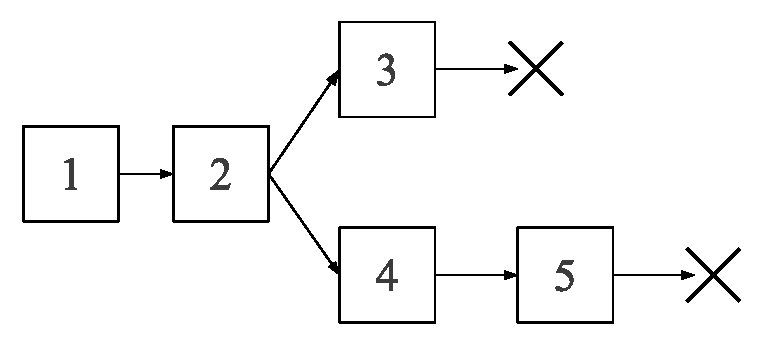
\includegraphics[width=0.4\linewidth]{pics/PST.eps}
	\caption{Дерево состояний вывода для формулы из примера \ref{proofexample}.}
	\label{fig:pst}
\end{figure}

На следующем рисунке представлено ДСВ, как связанные чанки.

\begin{figure}[h]
	%\vspace{0.5cm}
	\centering
	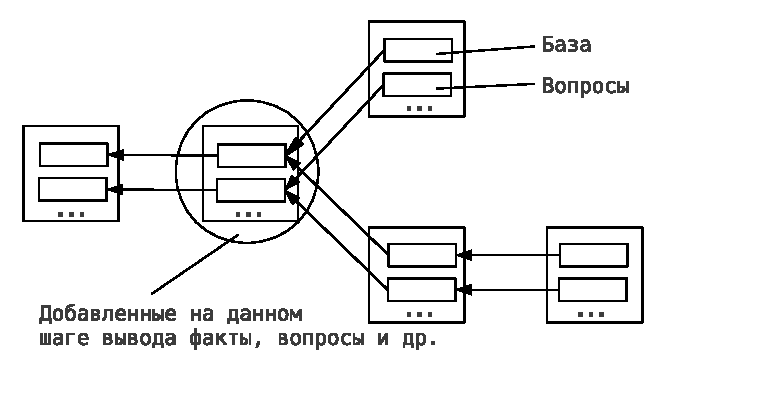
\includegraphics[width=0.6\linewidth]{pics/PST2.eps}
	\caption{ДСВ рис.~\ref{fig:pst}, \app{представленное в виде чанков}}
	\label{fig:pst2}
\end{figure}

\rem{С точки зрения реализации ДСВ растёт от листов к корню}{Не понял. Причем тут реализация? \app{М.б. это просто свойство структуры, как, например, в Linux директорий /var всегда растет.}}.

Для ДСВ реализована процедура схлопывания {\tt merge()}, преобразующая цепь узлов ДСВ в один узел. Это позволяет сократить используемую память, за счёт утраты подробной информации о шагах вывода, соответствующих цепочке узлов ДСВ.


%================================== СУПЕРВИЗОР =======================
\subsection{Супервизор}
Супервизор \que{наблюдает} глобально за всем ДСВ, обеспечивает алгоритмы информацией об ограничениях ресурсов, используемых эвристиках и т.п. В супервизоре находится список всех текущих листов ДСВ. Большинство стратегий реализовано на уровне супервизора, поскольку, в общем случае, необходимо использовать информацию о всей совокупности предшествующего или \rem{последующего вывода}{Вот коряво то, что прошлое и будущее симметричны... + Надо детально написать здесь, какая информация предоставляется эвристикам.}.

Наличие такого \rem{субъекта управления}{=СУпервизор, новая сущность?} обусловлено тем что некоторые частные события в процессе логического вывода могут повлиять на \rem{него}{Субъект или управление?} в целом.

%============================================================================
%================================== РАЗДЕЛЕНИЕ ДАННЫХ =======================
\subsection{Разделение общей оперативной памяти структурами данных}
Логический вывод, как правило связан, с получением новой дополнительной информации, ростом объема используемой оперативной памяти. Например, в метод Ррзолючии выводятся (синтезируются) новые дизъюнкты до тех пор пока не получится пустой дизъюнкт, а в методе доказательства ПО-формул производится насыщение баз фактами до тех пор, пока они не станут противоречивыми. Поскольку сложность формул может быть сколько угодно большой и даже минимальный вывод может иметь сколько угодно большую длину, имеет место проблема исчерпания имеющихся ресурсов вычислительной системы на хранение разрастающиеся структуры формулы. Опыт показывает \ref{reference}, что автоматический вывод довольно быстро занимает всю имеющуюся в распоряжении оперативную память, и далее процесс вывода требует регулярное удаление излишков. За излишки можно принять любые части формулы. Например, в системах основаных на методе резолюций удаляются дизъюнкты, которые либо вообще не участвовали в выводе, либо не участвовали в нём определённое количество шагов, иногда удаётся определить что дизъюнкт больше не пригодится. В случае ПО--формул, излишками являются устаревшие факты, фиктивные вопросы. Таким образом, проблема экономии оперативной памяти является важной, особенно с \que{учётом увеличения сложности задач}.

Для экономии памяти используются, во-первых проектирование компактных структур данных; во-вторых, методы разделения общих участков оперативной памяти (data sharing). В случае логических языков и конкретно языка ПО--формул использование методик хранения информации с разделением общей памяти является актуален. Исходя из некоторых общих особенностей представления языков первого порядка и представления ПО--формул, выделено и реализовано четыре методики разделения данных.

\rem{...}{Будем говорить о каком-либо специальном менеджере
  оперативной памяти?} (БУДЕМ)

\paragraph{Агрессивное разделение термов.} Заключается в том, что разделяются общие участки оперативной памяти среди термов. Например, в термах $A(g(a,f(x)),h(c))$ и $B(k,g(a,f(x)))$, подтермы $g(a,f(x))$ являются общими и представляют собой один и тот же участок в памяти. Данный подход позволяет достаточно экономить большие объемы оперативной памяти при ограниченных ресурсах, однако требует дополнительное процессорное время на вычисление общих подтермов. Такой метод является общеупотребимым в системах АДТ, классически варианты реализации представлены в \cite{}.

\paragraph{Мягкое разделение термов.} Отличается от агрессивного подхода намного меньшим потреблением процессорных ресурсов, но и меньшей эффективностью с точки зрения объема экономии памяти,
поскольку разделяет только часть общих подтермов. Исходя из определения \ref{ircond} применение правила вывода $\omega$ \app{корректно} в случае выполнения условия $A\theta \subseteq B$, где $A$ и $B$ соответственно конъюнкты вопроса и базы. Поскольку $B$ это уже существующее множество \rem{основных обобщенных термов}{Будем уточнять после вчерашнего разговора про НЭЭ?} (НЕТ), то для их хранения выделена соответствующая оперативная память. Подстановка $\theta$ же является отображением переменных вопроса $A$ в элементы эрбранова универсума. В дальнейшем при выполнении шага вывода $\theta$ применяется (апплицируется) ко всему консеквенту вопроса, и данный консеквент добавляется к формуле. Однако правая часть подстановки уже имеется в оперативной памяти в силу того, что основана она на термах из $B$. Исходя из этого, достаточно использовать ссылки на структуры и уже имеющуюся память, используемые для правых частей подстановки в тех частях консеквента, где эта подстановка применяется. 

Рассмтрим следующий фрагмент базовой ПО--формулы:

$$ \exists:A(f(e,g(t))) - \forall x:A(f(e,x)) - \exists:B(h(x),x) $$

В данном случае вопрос $\forall x:A(f(e,x))$ имеет ответ $\theta = \{x \rightarrow g(t)\}$. К базе фактов добавляется $B(h(x),x)\theta$, т.е. $B(h(g(t)),g(t))$. 

На рис.~\ref{datasharing1} представлен пример, демонстрирующий данную ситуацию с точки зрения мягкого разделения памяти.

\begin{figure}[h]
	%\vspace{0.5cm}
	\centering
	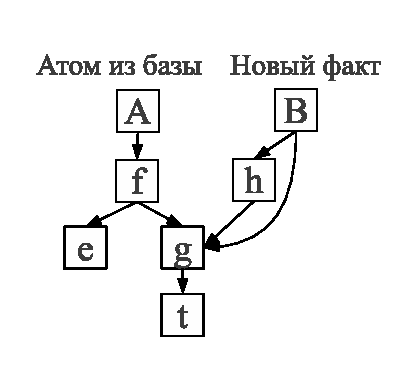
\includegraphics[width=0.3\linewidth]{pics/DataSharing1.eps}
	\caption{..}
	\label{fig:datasharing1}
\end{figure}

%------------Разделение по Черкашину------------
\paragraph{Разделение базовых подформул.} ПО--формулы, в которых производится ответ на вопрос с дизъюнктивным ветвлением, расщепляются на несколько новых базовых подформул. Количество новых базовых подформул совпадает с количеством непосредственных дизъюнктивных подформул в консеквенте вопроса. В простом варианте реализации ЛВ \cite{dissChe} такое расщепление требует копирования предыдущего состояния формулы несколько раз; такое копирование хотя и имеет линейную сложность \cite{Che2}, но всё равно естественно приводит к большим затратам памяти и процессорного времени, затрачиваемого для копирования. Разделение базовых подформул вполне реализуемо при помощи агрессивного разделения оперативной памяти термами. Однако, если формула предполагает достаточно сильное ветвление, сохраняется проблема наличия множества ссылок на разделяемые атомы баз, поскольку конъюнкт представляется как множество ссылок на атомы. Поскольку расщепление предполагает разделение общих частей баз, то имеет смысл разделять упомянутые выше ссылки. Данная стратегия реализуется за счёт средств ДСВ. Любая общая подветвь двух ветвей ДСВ является разделяемой. Рассмотрим небольшой пример.
 Пусть имеется следующая базовая подфомрула:
$$\exists: A(a) - \forall x: A(x) - \left\{
\begin{array}{lcl}
 \exists \colon B(x) & - & \forall y: B(y) - \exists\colon\boldsymbol{False}\\
 \exists \colon C(x) & - & \forall y: C(y) - \exists\colon\boldsymbol{False}
\end{array}
\right. $$

Обозначим первый и второй вопросы через $Q_1$ и $Q_2$ соответственно.

ДСВ для вывода данной формулы представлено на рис.~\ref{datahsaring2}.

\begin{figure}[h]
	%\vspace{0.5cm}
	\centering
	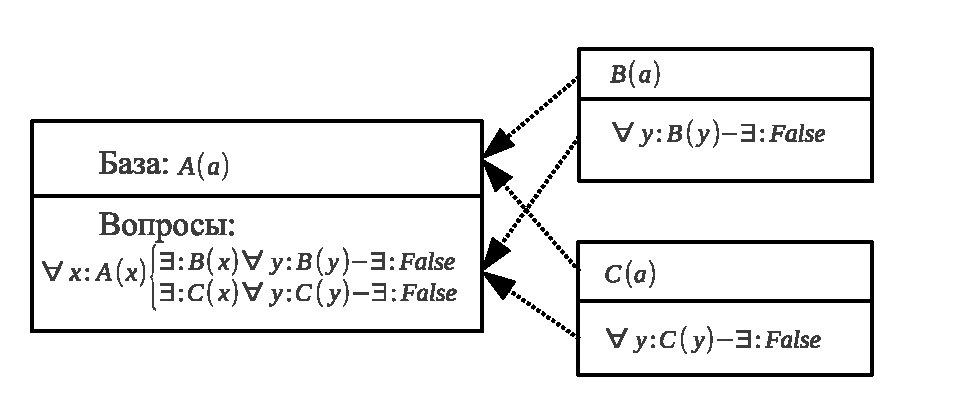
\includegraphics[width=0.7\linewidth]{pics/DataSharing2.eps}
	\caption{..}
	\label{fig:datasharing2}
\end{figure}

\paragraph{Разделение переменных и неопределенных эрбрановских элементов.} Данная методика предназначена для высокопроизводительного применения подстановки ко всей подформуле, т.к. все одноименные переменные в формуле представляют собой один участок в оперативной памяти. О неопределенных эрбрановских элементах сказано \rem{ниже}{А надо выше, после GTerm}. Все одноименные переменные на протяжении любого основного пути формулы \cite{dissChe} являются указателем на один и тот же участок в памяти. В отличие от агрессивного разделения данный подход учитывает роль переменных в процессе поиска ответных подстановок. В процессе применения подстановки переменная не заменяется на терм, а лишь указывает на этот терм, что позволяет экономить время на замену переменной термом в поддереве: достаточно одной операции присвоения над одной переменной, чтобы установить замену всех таких переменных в поддереве.


\paragraph{Удаление неиспользуемых фактов.} Ниже, показано что стандартная стратегия поиска ответных подстановок основано на том что каждого атома из конъюнктов вопросов производится попытка мэтчинга его с каждым атомов-фактом из базы. Поскольку, количество вопросов и длина конъюнктов конечны, то нетрудно определить для атома-факта из базы, мэтчится ли он хотя бы с одним атомом из вопросов. Если нет, то такой атом-факт можно удалить из базы, поскольку он вообще не используется в поиске ответных подстановок. Удаление ненужных фактов так же позволяет экономить память.

\paragraph{Веса подформул.} Под весом терма или подформулы понимается количество узлов в дереве, представляющем терм или подформулу. Анализ веса позволяет сдерживать разрастание формулы, и, соответственно обеспечить дополнительную экономию потребляемой памяти. Для этого из возможных ответов на вопрос приоритет отдаётся тому, который приводит к формуле наименьшего веса.

\rem{...}{Что насчет управления комбинациями методик? Откат и вес? Как задавать эти комбинации? ли это уже реализация, наверное.}


%================================== ОГРАНИЧЕНИЕ РЕСУРСОВ =======================
\subsection{Стратегия ограниченных ресурсов}
Стратегия ограниченных ресурсов реализована в большинстве современных систем АДТ, в том числе и в Вампире \cite{}. В данной системе подобная стратегия \que{напрямую} зависит от текущего ДСВ и описывается следующим образом. Ветка ДСВ растет до тех пор, пока не наступит ограничение объема оперативной памяти, разрешенной для использования, либо пока не исчерпается определенное время, либо пока не будет произведено определенное количество шагов вывода. Если наступил предел использования ресурсов, то осуществляется откат назад и выбор других ответов, т.е. используются другие варианты построения дерева.

%======================== INDEXING ===========================
\subsection{Индексирование данных}

Формализации некоторых задач могут быть довольно обширными, например задача ALG214+4 из библиотеки TPTP в языке ПО--формул занимает порядка 10мб. Кроме того, даже если изначальная формула не столь велика, после некоторого количества шагов вывода, она может разрастись до сколь угодно большого размера. Стратегии разделения данных позволяют лишь отсрочить момент переполнения памяти, а так же вместить в имеющуюся память формулу как можно большего размера. 

С другой стороны существуют ситуации, когда необходимо анализировать ПО--формулу на наличие определённых свойств. Такой анализ проводится как в рамках логического вывода, так и отдельно. Например, если для задачи заданна некоторая стратегия вывода, то для осуществления очередного шага вывода выбирается ответ, а значит база и вопрос, соответствующий этой стратегии, т.е. анализируется вся формула, и выбираются удовлетворяющие тратегии части формулы. Кроме того анализ формул часто требуеться после вывода формулы, для сбора статистики и другой информации, позволяющей в дальнейшем разрабатывать новые стратегии, либо извлекать содержательную информацию из ЛВ.

Отсюда необходимо разработать методы, позволяющие в формуле производить эффективный поиск необходимых её (термов, вопросов, овтетов). Для решения данной проблемы обратимся к существующему опыту.    

%индексирование термов
\paragraph{Индексирование термов}
Основной структурой, используемой для представления формул является обобщенный терм. Он используется для представления элементов конъюнктов, кванторных переменных, обеих частей подстановок. Поэтому актуальной задачей является эффективный поиск обобщенных термов в формуле по заданным критериям.

В информационных технологиях поиск данных часто разрешаются, например, с помощью методов индексирования данных, применяемых широко в реляционных базах данных \cite{Ulman}. 

В нашем случае основной объект индексирования --- это обобщенный терм, который является древовидной структурой, индексирование которой методами, используемыми в  реляционных БД, неэффективно \cite{Graf}. Поэтому используются нижеописанные подходы.

Индексирование термов к настоящему времени хорошо исследовано, как в рамках определенных систем АДТ, так и абстрактно. В частности по данной теме существует ряд интересных работ, в том числе [дискриминационное дерево и пути, подстановочное дерево, и книжку Графа про индексирование]. \app{Представленные в этих работах методы}, позволяют эффективно находить в базе термов те термы, которые удовлетворяют определенным критериям: являются равными данному (query term), являются его примерами, обобщениями (generalization) и унификациями. Для наших нужд не требуется \rem{обобщение и классическая унификация}{Обновить надо?}, но дополнительно необходимы методы индексной поддержки НЭЭ-унификации: критерий наличия термов, включающих заданный подтерм; различные количественные критерии: вес, глубина, арность. С учетом перечисленных требований а также того факта, что как правило, в базе находятся основные \rem{термы}{Через абзац будет использоваться ``основной пример'' кругом.}, качестве основы методики индексирования выбрано индексирование путями []. Кратко опишем её суть, как она описана в [].

Для каждого символа входящего в терм составляется список так называемых \emph{путей}. Путь --- это последовательность чередующихся символов и чисел, где число определяет позицию символа среди дочерних узлов \cite{disctree}. Например, атом $A(e,f(f(x,k),y),m)$ представляется в виде путей $A$, $A1e$, $A2f$, $A2f1f$, $A2f1f1x$, $A2f1f2k$, $A2f2y$, $A3m$. То есть каждому символу соответствует путь от корня до этого символа в древовидном представлении обобщенного терма. Подробнее на рис.~\ref{pathfig}. Каждый из этих путей содержит указатель на соответствующий терм, т.е. тот терм для которого строился путь. Сами пути хранятся в отсортированном виде (в дереве).

\begin{figure}[h]
	%\vspace{0.5cm}
	\centering
	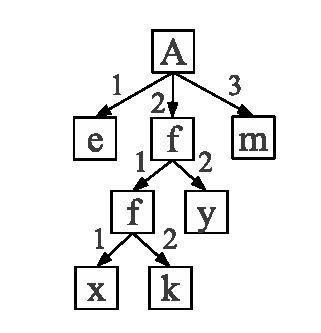
\includegraphics[width=0.2\linewidth]{pics/Path1.eps}
	\caption{..}
	\label{pathfig}
\end{figure}

Пример. Пусть дан атом $A(a,f(x,b))$ и множество атомов $\{A(a,f(c,b)), A(a,f(b,e)),A(a,f(k,b)), A(b,f(e,b))\}$. Любой атом, являющийся основным примером для заданного, содержит в своём списке путей следующие пути: $A1a$, $A2f2b$. Таким образом, для поиска основных примеров заданного атома необходимо найти пересечение множеств атомов, на которые указывают пути.  В частности путь $A1a$ указывает на множество $\{A(a,f(c,b)), A(a,f(b,e)),A(a,f(k,b))\}$, а путь $A2f2b$ на $\{A(a,f(c,b)), A(a,f(k,b)), A(b,f(e,b))\}$. Пересечение этих множеств есть множество $\{A(a,f(c,b)),A(a,f(k,b))\}$, это и есть множество примеров для атома $A(a,f(x,b))$. 

Методы индексирования термов в настоящее время широко используются во многих известных системах АДТ [Vampire -улучшенное индексирование путями, Otter -дискр.дерево и пути, E, EQP, SPASS -дерево подстановок].

Кроме базы термов, в индексировании нуждаются множества вопросов и множества ответных подстановок. Поскольку количество вопросов не так велико как количество термов, то достаточно использовать возмодности обычного словаря.

%индексирование других частей формулы
\paragraph{Индексирование других частей формулы}
Теперь опишем другие \app{проблемы, решаемые при помощи} индексирования. Предположим что \rem{пользователем}{Надо про него   что-то сказать, хотя бы во введении. Его участие в АДТ.} задана некоторая стратегия для решения некоторого класса задач. Стратегия оперирует вопросами с определенными свойствами (т.е. вопросу сопоставляется содержательная информация), которые присущи всему классу задач (т.е. все задачи объединяет наличие определенных вопросов). Для повышения производительности поиска ЛВ необходимо упростить в дальнейшем доступ к таким вопросам, чтобы каждый раз повторно не проверять  все вопросы на наличие определенного свойства. Для этого достаточно сделать словарь (map) в котором каждому \rem{описанию вопроса}{Что за описание? как оно соответствует критериям и индексированию? Это реализовано? Если да, то почему в сослагательном наклонении?} соответствовал бы указатель на данный вопрос. \rem{В принципе, в стратегиях задавать опции при помощи номеров вопросов, но тогда теряется гибкость: пользователю необходимо ставить вопросы всегда на одно и тоже место. Данный вид индексирования (весьма простого) может выполняться как на этапе компиляции (тогда в компиляции прувера будет задействован не только стратегия но и сама задача), так и при первичном обращении к вопросу (тогда нет необходимости в компилировании самой задачи).}{О чем это?}


\paragraph{Индексирование ПО--формул} Доказательство крупных формул может производиться в несколько этапов, с сохранением промежуточных результатов на жесткие носители информации. Сам вылогический вывод формально является цепочкой формул. Для анализа описанных ситуаций необходимо проверять формулы на наличие некоторых свойств. Поскольку, ПО--формула как и обобщенный терм имеет древовидную структуру, то для её индексирования применимы описанные выше методы индексирования путями. Однако в данном случае индекирование путями требует доработки, поскольку, в случае термов путь однозначно задавался символами и номерами дочерниих узлов, то в случае ПО--формул номера дочерних узлов сохраняются, а вот символу может соответствовать любая формально описуемая характеристика узла ПО--формулы (типового квантора). [Буду дописывать данный параграф. Есть поле для размышлений. Можно на статью небольшую сделать. В книгах про индексирование подобные задачи описаны как нужные.] 


%================================== ЛЕНИВАЯ КОНКРЕТИЗАЦИЯ =======================
\subsection{Неограниченные переменные}
Проблема неограниченных переменных описана выше. Кратко опишем её суть. Согласно определению \ref{ircond}правило вывода $\omega$ применимо в том случае если вопрос $\forall \bar{y}\colon A$ к базе $\exists \bar{x}\colon B$ имеет {\em ответ} $\theta$  такой что $\theta$ есть подстановка $\bar{y} \rightarrow H^{\infty}$ и $A\theta \subseteq B$. В случае если все перменные из $\bar{y}$ содержатся в конъюнкте $A$, то поиск соответствующих элементов из $H^{\infty}$ производится с помощью алгоритма поглощения. Если же среди $\bar{y}$ имеются переменные, которые не входят в $A$, то такие переменные называются \emph{неограниченными}, и не используются в алгоритме поглощения. Но подстановка для них необходима, причём любой элемент эрбранова универсума является формально корректной подстановкой. Проблема в том, что в общем случае (при наличии функциональных символов) эрбранов универсум является бесконечным множеством, и какой именно элемент из него необходимо выбрать неизвестно.

Решение данной проблемы не является тривиальной. Нами предложенно несколько подходов.

\subsubsection{Стратегия ленивых конкретизаций}
Суть ленивой конкретизации заключается в следующем. В качестве подстановки для неограниченной переменной выбирается не конкретный элемент эрбранова универсума, а неопределенный эрбрановский элемент (НЭЭ), который, в дальнейшем, исходя из нужд вывода, постепенно конкретизируется до основного терма, либо в некоторых ситуациях так и остается недоопределенным. Поясним некоторые слова из предыдущего предложения. В данном случае <<нужды вывода>> это возможность ответа на вопрос, и НЭЭ конкретизируется таким образом, что бы появился новый ответ на вопрос, т.е. решается следующая задача: до какого терма конкретизировать НЭЭ, что бы появился ответ на вопрос?. Отметим, что НЭЭ первоначально появляется как часть ответа в одном вопросе, а его конкретизация производится при поиске ответов на другие вопросы. Под <<постепенной конкретизацией>> понимается процедура ленивых вычислений: НЭЭ доопределяется на столько точно, на сколько этого достаточно для ответа на текущий вопрос, т.е. конкретизация может быть неполной (т.е. не конкретизирующая НЭЭ до основного терма), например НЭЭ $h$ конкретизируется до $f(h_1)$, где $h_1$ новый НЭЭ. 

По своей природе НЭЭ схож со [\app{свободной}] переменной в том смысле, что он \rem{изменяем}{Уточни термин.}, однако все такие изменения должны быть направлены \app{только} на конкретизирова\app{ние} НЭЭ, т.е. НЭЭ заменяется только на некий терм (возможно тоже содержащий НЭЭ), либо на другой НЭЭ, но не на переменную. Однако, при замене переменной на НЭЭ, НЭЭ обладает \app{всеми} свойствами терма.

Рассмотрим пример приложения этой техники в процессе построения логического вывода для следующей формулы.
\begin{equation}
	\forall\colon\boldsymbol{True} - \exists\colon\boldsymbol{True} -
	\left\lbrace
	\begin{array}{l}
		\forall x\colon\boldsymbol{True} - \exists\colon A(x) \\
		\forall x\colon A(f(x)) - \exists\colon B(f(x)) \\
		\forall\colon B(f(a)) - \exists\colon \boldsymbol{False}
	\end{array}\right.
\end{equation}
На первом шаге вывода получен ответ $\{x \rightarrow h_1\}$ на первый вопрос, $x$ является неограниченной переменной, $h_1$ --- это неопределённый эрбрановский элемент (НЭЭ). После первого шага атом $A(h_1)$ добавляется в базу. На втором шаге вывода получен ответ $\{x \rightarrow h_2\}$ на второй вопрос, и $h_1$ конкретизируется до $f(h_2)$, после второго шага $B(f(h_2))$ добавляется в базу. Наконец, на третьем шаге получен тривиальный ответ на третий вопрос, и $h_2$ доопределяется до $a$.

Однако существуют особые ситуации. Рассмотрим следующий пример.
\begin{example}[]\label{example:uhe1}
$$\fictAquantor \; - \; \exists\colon M(e) \left\{
\begin{array}{lcl}
 \forall x,y\colon M(x) & - & \exists\colon S(y),M(f(x)),T(x) \\
 \forall x \colon T(x),S(e) & - & \exists\colon Q(x) \\
 \forall x \colon Q(x),S(f(e)) & - & \exists\colon\textbf{False}
\end{array}
\right.$$

Данная формула имеет вывод, например такой. Получаем ответ на первый вопрос подстановкой $\{ x\rightarrow e, y\rightarrow e \}$, в результате в базу попадают факты $S(e),M(f(e)),T(e)$; ответ на второй вопрос есть $\{ x \rightarrow e\}$, и в базу попадает $Q(e)$; полученных фактов в базе недостаточно для ответа на целевой вопрос, поэтому вновь отвечаем на первый вопрос, при этом возможно несколько вариантов ответа, но, что важно, переменную $y$ необходимо заменить на $f(e)$. Выберем, например, следующий ответ $\{x \rightarrow e, y \rightarrow f(e) \}$ и в базу попадет факт $S(f(e))$ после чего на целевой вопрос ответ получается. Заметим, что на первый вопрос необходимо обязательно выбирать те подстановки, которые содержат $y \rightarrow e$ и $y \rightarrow f(e)$, они необходимы для ответа на второй и третий вопросы, соответственно. Формула устроена таким образом что первый и второй вопросы всегда имеют новые ответы.

Теперь рассмотрим работу стратегии ленивой конкретизации. Ответ на первый вопрос будет следующего вида $\{ x\rightarrow e, y\rightarrow h_1 \}$, где $h_1$ --- НЭЭ, и в базу попадают следующие факты $S(h_1),M(f(e)),T(e)$. Ответ на второй вопрос --- $\{ x\rightarrow e, h_1\rightarrow e \}$, в котором $h_1$ доопределяется до $e$, и, соответственно, находящийся в базе факт $S(h_1)$ доопределяется до $S(e)$. С этого момента начинается выполнение, фактически, циклической операции, поскольку целевой вопрос не имеет ответа: вновь получаем ответ на первый вопрос, и вновь в базу попадает факт $S(h_1)$, который при ответе на второй вопрос вновь доопределится до $S(e)$ и т.д. Однако если пропустить ответ на второй вопрос, то при ответе на целевой, факт $S(h_1)$ доопределится до $S(f(e))$ и на этом вывод закончится.
\end{example}


В общем виде проблема заключается в том, что существуют ситуации, когда с формальной точки зрения НЭЭ конкретизируется корректно, но не там где это требуется, например раньше, чем это необходимо при ответе на другой вопрос. Либо НЭЭ может конкретизироваться там где это уже не требуется. Из подобных примеров видно, что ленивая конкретизация не может использоваться на прямую. Необходимы дополнительные средства обеспечения логического вывода, учитывающие описанные только что проблемы. 

%\rem{...}{Надо подработать этот абзац. Написать точнее: Доопределяется не так как требуется,... не там, где необходимо.}

%------------первый вариант
\paragraph{Ограничение количества конкретизаций}
Два НЭЭ будет называть \emph{подобными}, если они получены в результате выбора подстановки для одной и той же переменной. Такая ситуация имеет место быть если на один и тот же вопрос с неограниченными переменными произведено несколько ответов, для неогарниченных переменных все разы в качестве подстановки выступает новый НЭЭ.

Ограничение одинаковых конкретизирований для подобных НЭЭ позволяет исключить ситуации, когда НЭЭ доопределяется там где это уже не требуется, и как следствие появляется возможность конкретизировать его в другом месте. Для каждого НЭЭ хранится ссылка на переменную, для которой этот НЭЭ был выбран как подстановка. В вопросах, каждой неограниченной переменной соответствует набор термов, до которых доопределялись НЭЭ соответствующие данной переменной. Таким образом имеется возможность отслеживать сколько раз и до чего конкретизировался данный НЭЭ. Если лимит конкретизаций закончен, то процедура матчинга заканчивается неудачей. Выбор конкретного числа, ограничивающего количество конкретизаций, определяется либо пользователем исходя из его знаний о задче, либо это число изначально устанавливается равным 1, и далее в случае неуспешности вывода за определенное количество шагов или времени, это число увеличивается.

Использование данного подхода позволяет решить пример \ref{example:uhe1} за 5 шагов, если установить единице лимит конкретизаций для переменнй $y$ из первого вопроса. Посольку $h_1$ не будет конкретизироваться до $e$ второй раз, во втором вопросе. 

%--------------------ещё вариант
\paragraph{Сохранение выражений, содержащих НЭЭ}
Представим другой вариант управления стратегией ленивых конкретизаций. Описанный выше вариант конкретизаций НЭЭ, в том числе используемый в примере \ref{example:uhe1}, не сохраняет исходное выражение, содержащийся в котором НЭЭ конкретизируется. Отсюда возникает проблема потери информации. Например, если в примере \ref{example:uhe1} в базу попадает атом $S(h_1)$, то при необходимости конкретизации $h_1$, конкретизация производится не в самом атоме, а пораждается новый атом, такой, как если бы был конкретизирован исходный, т.е. в случае рассматриваемого примера, к базе добавляется атом $S(e)$, при этом атом $S(h_1)$ сохраняется. НЭЭ $h_1$ сохранён, а значит может использоваться в других вопросах.

Содержательно такой подход означает следующее. Можно считать что для вопроса с открытыми переменными применяется вся совокупность возможных ответов, т.е. с использованием всех элементов эрбрановского универсума. Понятно, что это технически нереализуемо из-за бесконечности эрбановского универсума, то используется техника ленивых вычислений. В идеале предполагается, что за один раз используются все возможные ответы на вопрос, но на самом деле используются только необходимые в определёной ситуации. Например, если в некоторой формуле содержится вопрос $\forall x: True  - \exists A(x)$, и $H^{\infty}= \{a, f(a), f(f(a)), ...\}$, то использование всех возможных ответов разом приводит к попаданию в базу элементов $\{A(a), A(f(a)), A(f(f(a))), ...\}$, которых бесконечно много. Вместо этого множеству ставится в соответствие элемент $A(h)$, где $h$ --- НЭЭ, и в дальнейшем этот элемент пораждает необходимые элементы множества. 

В данном случае можно заметить сходство со стратегией ленивых конкретизаций, без каких-либо ограничений. Преимущество данного подхода заключается в том, что выражение, содержащее НЭЭ всегда сохраняется, т.е. не может быть утрачено за счёт <<неугодных подстановок>>. 

Рассмотрим отдельно два случая. Если конкретизируемый НЭЭ содержится в подформуле-вопросе, и если конкретизируемый НЭЭ первоначально появился после ответа на вопрос с дизъюнктивным ветвлением. 

В случае с дизъюнктивынм ветвлением, вся совокупность оветов на вопрос означает не просто появление бесконечного конъюнкта, а бесконечно множества конъюнктов, поскольку база ещё и расщепляется. Т.е. конкретизация НЭЭ приводит не просто к пораждению нового атома в конъюнкте, а к очередному расщеплению формулы, в той точке логического вывода, в которой впервые появился доопределяемый НЭЭ. Данную точку легко отследить благодаря структуре ДСВ, в которой сохраняются все события произошедшие на каждом шаге вывода. Однако, ветвление целесообразно проводить не в этой точке, а во всех листах дерева, корнящегося из этой тчоки. Поскольку вставка втевления в середину вывода потребует копирования для каждого нового узла той части вывода которая была уже прозведенаа.  На рис.~\ref{lazy21} схематично показано некоторое ДСВ.

\begin{figure}[h]
	%\vspace{0.5cm}
	\centering
	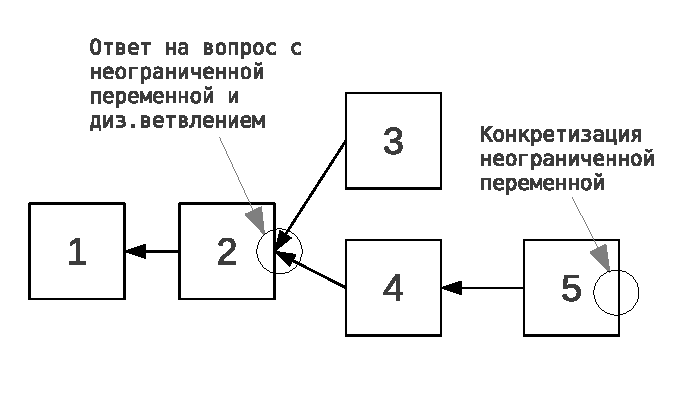
\includegraphics[width=0.5\linewidth]{pics/Lazy21.eps}
	\caption{..}
	\label{lazy21}
\end{figure}

После конкретизации НЭЭ, получаем структуру ДСВ, изображенное на рис.~\ref{lazy22}

\begin{figure}[h]
	%\vspace{0.5cm}
	\centering
	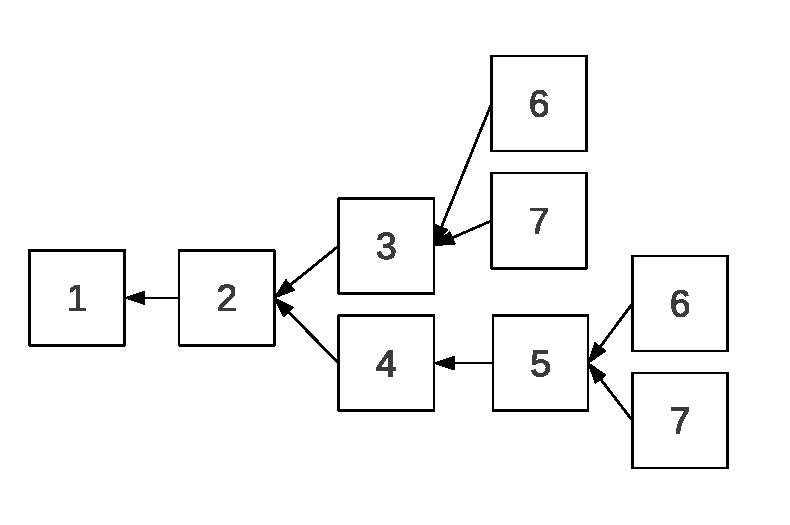
\includegraphics[width=0.5\linewidth]{pics/Lazy22.eps}
	\caption{..}
	\label{lazy22}
\end{figure}

В случае подформулы-вопроса, содержащего НЭЭ, конкретизация НЭЭ требует пораждения новой подформулы-вопроса, отличающейся от исходной только в точке содержания НЭЭ. Возможно появление множества вопросов, усложняющее в целом структуру формулы, и её вывод. Под усложнением структуры в данном случае понимается именно наращивание количества вопросов. Абсолютный размер формулы (в байтах) меняется незначительно, поскольку используются стратегии экономии памяти. Новую подформулу-вопрос целесообразно вставлять в той точке вывода (перед этим узлом), где первоначально добавился вопрос с НЭЭ. Предположим что на рис.~\ref{lazy21} вопрос с НЭЭ впервые появляется в узле 2. Тогда если конкретизация НЭЭ потребуется в любом из последующих узлов, дерево преобразуется в вид, как на рис.\ref{lazy23}. При этом новый узел 6 содержит только новый пораждённый вопрос.

\begin{figure}[h]
	%\vspace{0.5cm}
	\centering
	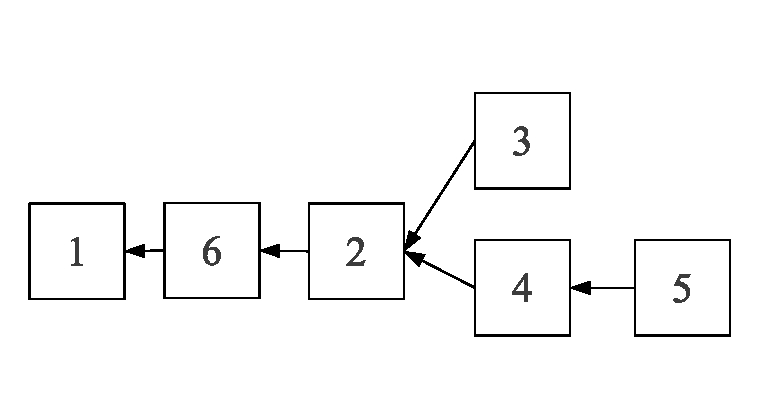
\includegraphics[width=0.5\linewidth]{pics/Lazy23.eps}
	\caption{..}
	\label{lazy23}
\end{figure}


%---------------второй вариант
\paragraph{Ручное управление}
Одним из вариантов решения проблемы является использование языка описания стратегий, с помощью которого можно, например, указать, что на второй вопрос необходимо ответить лишь один раз, либо использовать на первый вопрос сразу несколько подстановок содержащих $y\rightarrow h_1$ и $y\rightarrow h_2$. Это приведет к попаданию в базу двух фактов $S(h_1)$ и $S(h_2)$, один, из которых будет использоваться для второго вопроса, а другой для целевого. Такой вариант вполне приемлем, и предполагается что именно он и будет чаще всего использоваться для решения задач. \app{Такой подход в настоящее время пока не обеспечивает принципиальную выводимость, но для отдельных классов задач .....} \rem{Но что делать, если дополнительные знания о задаче не позволяют сформулировать правильную стратегию? Необходимо предоставить хотя бы принципиальную возможность вывода, что пока необеспеченно.}{Удалить м.б.}

%-------------
Отметим, что стратегии, основанные на использовании НЭЭ, \rem{стоят особняком}{Уточни. Конфликтуют или не конфликтуют, вмешиваются или не могут быть скомплексированы??} для многих других стратегий. Во-первых, при использовании этой стратегии нарушается независимость базовых подформул, поскольку один и тот же НЭЭ может быть в разных подформулах: доопределение общего НЭЭ в одной подформуле автоматически приводит к доопределению его в другой подформуле. Этот факт, в частности, делает зависимыми процессы поиска ЛВ в базовых подформулах на параллельных вычислительных архитектурах. Он также противоречит некоторым эвристическим уточнениям алгоритмов и стратегий, например, {...}{Пошел простой пример стратегии.}.

\subsubsection{Cтратегия фильтрации эрбрановского универсума}
Другим вариантом (помимо стратегии ленивых конкретизаций) решения проблемы неограниченных переменных, является стратегия фильтрации эрбрановского универсума. Данная стратегия позволяет избавиться от изложенных в начале главы проблем, но несколько расширяет пространство возможных ответов. Суть данной стратегии заключается в следующем. В консеквентах, атомы, которые содержат неограниченные переменные вопросов, должны унифицироваться с одноимёнными атомами из всех других частей всей базовой подформулы, в противном случае атом попавший в базу не будет удовлетворять условию применения правила вывода (\ref{irond}), поскольку никода не выполнится процедура матчинга при поиске ответов. Будем использовать данное свойство в стратегии. В качестве ответа для неограниченных переменных используются такие термы, что атом полученный подстановкой переменных на эти термы будет основным примером найденной унификации. Такой подход позволяет заранее сузить пространство эрбрановского универсума, фильтруя заведомо бесполезные ответы.

Для ясности рассмотрим пример. Пусть имеется следующие вопросы ПО--формулы.

$$Q_1 = \forall x,y: - \exists: A(f(x,g(y)))$$
и
$$Q_2 = \forall x:A(f(e,x)) - \exists: False$$

В данном случае в консеквенте вопроса $Q_1$ содержится атом $A(f(x,g(y)))$. Одноимённый атом для данного, это атом вопроса $Q_2$, а именно $A(f(e,x))$. Унификация двух данных атомов есть $A(f(e,g(y)))$. Основной пример данного атома есть любой, атом полученный из исзодного заменой переменной $y$ на любой элемент $H^{\infty}$. Тогда ответ для вопроса $Q_1 = \{x \rightarrow e, y \rightarrow t\}$, где $t$ любой элемент $H^{\infty}$, например $e$. В базу попадёт факт $A(f(e,g(e)))$ и ответ на целевой вопрос будет $\{x \rightarrow e\}$. 

Такой подход имеет сходство со стратегий ленивых конкретизаций, в которой конкретизация НЭЭ по сути означает сужение эрбранова универса, до множества основных примеров конкретизации. В данном же случае ограничения на ЭУ накладываются сразу, исходя из потенциальных вопросов. В случае стратегии ЛК, конкретизация как раз производится при поиске ответов на эти потенциальные вопросы. 

Данная стратегия позволяет всегда работать с полностью конкретизированной формулой, т.е. формулой не содержащей НЭЭ.


%=============================================================================================
%======================================================================
%================================== k,m-ограничение =======================
\subsection{Стратегия $k,m$--ограничения}
Данная стратегия формулируется следующим образом. Некоторый ответ применяется, если за последующие $k$ шагов произойдет заданное событие по меньшей мере $m$ раз. Пользуясь терминологией ДСВ, это означает что для данного узла дерева применяется ответ в случае, если построенное в результате дальнейшего вывода поддерево коренящееся с этого узла не превысит глубину $k$ и до этого момента произойдет $m$ раз заданное событие. Предложено три спецификации данной стратегии.

\paragraph{$k,m$--опровержение.} Заданный ответ выбирается в случае, если за последующие $k$ шагов ЛВ будет опровергнуто как минимум $m$ баз. Подобная стратегия, а именно $k$--опровержение, первоначально предложена в \cite{ICDS2000} и реализована в системе КВАНТ/1 Черкашина Е.А. \cite{dissChe}, где показана её состоятельность. В данной системе эта стратегия расширена вторым параметром $m$. Она позволяет сдерживать разрастание пространства поиска вывода, т.е., сдерживает излишнее ветвление ДСВ, что в некоторых случаях приводит к многократному усложнению вывода.

Отметим, что выбор параметров $k$ и $m$, заранее не определён, и пользователю необходимо знать следующие нюансы. Во-первых, параметр $k$ означает что будут проверены все возможные ответы на глубине $k$ шагов, т.е. произведен полный перебор, что в свою очередь может затратить большие ресурсы процессорного времени и памяти. Параметр $m$ дополнительно усиливает, условие выбора исходного ответа. Поэтому если заранее нельзя предположить какие выбрать эти параметры, по умолчанию они устанавливаются $k=1$ и $m=p$, где $p$ количество непосредсветнных дочерних дизъюнктивных узлов вопроса, и в случае неудачи ЛВ, параметр $k$ постепенно увеличивается, а $m$ уменьшается.

\paragraph{$k,m$--конкретизация.} Иная спецификация стратегии $k,m$--ограничения, формулируется так. Ответ на вопрос принимается, если за последующие $k$ шагов будет доопределено $m$ НЭЭ. Эта стратегия также направлена на то чтоб ограничить сложность представляемой формулы. С недоопределенным НЭЭ ассоциируется много дополнительной информации и условий, описанных в главе о неограниченных переменных, что на уровне реализации влияет негативно. Поэтому чем больше и быстрее НЭЭ будут доопределены, тем лучше. 

\paragraph{Особенности реализации стратегии $k,m$--ограничения}
Основной для реализации данной стратегии являются описанные выше ДСВ и супервизор. Параметры $k,m$ и собственно условие задаются в супервизоре и привязывается к определённом узлу ДСВ. Супервизор проверяет все условия на каждом шаге ЛВ. И в положительном случае (когда условие выполнено) производится возврат поиска (backtracking) назад, т.е. производится последовательное удаление узлов дерева в обратном порядке (от листа в направлении корня). Перед удалением каждого узла производится разконкретизация НЭЭ, полученных в этих узлах и возврат использованных вопросов в стадию активных (т.е. возможных для применения).

%================================== КЕШИРОВАНИЕ =======================
\subsection{Кэширование результатов}
Учитывая множественность возможных ответов, возвратов поиска в выводе, большой глубины вывода, большого количества атомов в базе и т.д. целесообразно кешировать некоторые результаты чтобы не производить снова повторяющиеся вычисления.

Добавление уже имеющихся в базе атомов не допускается. Поэтому процедура поиска ответов работает всегда с новыми атомами, и производит всегда новые вычисления. Тем не менее полученные ответы в итоге могут совпадать. Все примененные ответы сохраняются, причем хранятся они как и база в чанках, расположенных по всему пути от листа до узла. Это позволяет делать корректные возвраты поиска с учетом сохранения информации о примененных ответах.

\rem{...}{Тут можно было б таки описать, как кэш используется. Что строиться - понятно. А как используется и где, когда, не понятно.}

%-----------PARALLEL STRATEGY---------------------------
\subsection{Параллельные стратегии}

Повышать производительность можно при помощи вышеописанных интенсивных методов, ориентированных на оптимизацию использования вычислительных ресурсов, а также при помощи экстенсивных методов, базирующихся на вовлечении в процесс дополнительных вычислительных ресурсов. В частности, это становится актуальным ввиду широкого распространения многоядерных вычислительных систем общего назначения, в частности, рабочих станций. Одним из популярных экстенсивных методов повышения производительности является разработка версий программ АДТ для кластерных архитектур в параллельном режиме исполнения ветвей подпрограмм. Рассмотрим методики и стратегии построения параллельных реализаций алгоритмов поиска ЛВ в исчислениях ПО--формул.

Предложены следующие стратегии для построения параллельных схем алгоритмов поиска логического вывода.

\paragraph{Первая стратегия}

В случае, если вопрос имеет дизъюнктивное ветвление, то после ответа на этот вопрос, формула расщепляется и трансформируется в формулу с б\'{о}льшим количеством баз, т.е. в общем случае, количество базовых подформул увеличивается с каждым шагом вывода. С другой стороны, исходная формализация задачи в языке ПО--формул, опять же в общем случае, содержит более одной базовой подформулы. Для того, что бы показать, что исходная формула противоречива, необходимо опровергнуть каждую из баз. Специфика исчисления ПО-формул, позволяет производить логический вывод и опровержение этих баз независимо друг от друга. Данное свойство называется естественным ИЛИ-параллелизмом [], который следует из того что в базах находятся лишь основные термы. Поэтому процедура опровержения каждой базы может выполняться в отдельном вычислительном процессе или на отдельном вычислительном устройстве.

Таким образом, первая стратегия, реализуемая в виде параллельной схемы алгоритмов, формулируется следующим образом: каждая базовая подформула \app{, содержащая только основные термы в базе,} опровергается независимо от других базовых подформул, а значит для этот процесс выделяется в отдельный параллельный независимый от других процесс, синхронизируемый с другими процессами только  на этапах его создания в момент расщепления формулы и завершения в момент установления выводимости/невыводимости. Во время жизни этого процесса к нему может поступать асинхронный сигнал завершения от супервизора, обозначающий, что выполнение процесса далее не имеет смысла, например, формула является неопровержимой, что было доказано в какой-либо другой ветка поиска доказательства, или пользователь остановил выполнение программы. Для программной реализации алгоритмов данной стратегии созданы подпрограммы жесткого копирования и \rem{маршаллинга/демаршаллинга}{Представления динамической памяти в таком виде, чтобы была возможность передать ее состояние через сеть, и, далее восстановить в другом процессе.} (следующая глава), что бы полностью скопировать базовую подформулу и обрабатывать её в отдельном процессе независимо, т.е. не разделяя оперативную память.

\rem{...}{Думаю этот раздел немного покажет тебе на сколько подробно можно и надо писать.}

\paragraph{Вторая стратегия}
Для применения каждого шага логического вывода, необходимо выполнять, в общем случае, поиск ответных подстановок для заданного вопроса. Поиск ответных подстановок не изменяет структуру формулы, и не использует общих изменяемых данных, это значит, что процессы поиска ответа на каждый вопрос независимы, а значит параллельны. \rem{...}{М.б. тут тоже рассказать в общих чертах о варианте реализации, например, что это не будет отдельный процесс или узел, а будет поток (нить)}


\paragraph{Третья стратегия}
Теперь рассмотрим процедуру поиска подстановок для отдельно взятого вопроса. Как было сказано во введении, подстановка $\theta$ является ответом, если выполняется условие $A\theta \subseteq B$, где $B$ --- конъюнкт вопроса, $A$ --- конъюнкт базы. Для сохранения полноты необходимо хотя бы потенциально иметь в распоряжении все возможные ответы, из которых выбирается подстановка для данного шага. Ниже описана структура хранилища ответов. Можно говорить о том что наполнение каждого чанка хранилища подстановками производится параллельно, поскольку чанки независимы.

\paragraph{Свойства стратегий}

Анализ, описанных выше стратегий, показывает, что они обладают свойством вложенности. Т.е., для того, что бы опровергнуть одну базовую подформулу (первая стратегия) необходимо найти ответы на вопросы (вторая стратегия). В свою очередь для поиска ответа, необходимо найти подстановки для каждого атома из конъюнкта вопроса (третья стратегия).

Исходя из этого, данные стратегии можно разместить по степени эффективности (иерархия стратегий). Не трудно видеть, что время, затрачиваемое на опровержение базы, как минимум, не меньше, чем время, затрачиваемое на поиск ответных подстановок, а на практике, как правило, оказывается намного больше, так как для опровержения базы необходимо неоднократно ответить на некоторые вопросы. Аналогичные выводы делаются по отношению к другим стратегиям.

Кроме того, можно выделить единое для всех стратегий свойство – свойство однородности. Т.е. стратегии имеют единую структуру. А именно, все они, по сути, сводятся к применению некоторой операции (опровержение базы, поиск ответов и т.д.) для каждого элемента некоторого множества (базы, вопросы и т.д.).

Одной из рекомендаций при реализации описанных алгоритмов на кластерных вычислительных системах является правильное распределение задач между вычислительными узлами кластера, в зависимости от скорости коммуникации между ними. Например, программная реализация первой стратегии должна процесс привязывать к вычислительному узлу. Однако этого не стоит делать при реализации остальных стратегий, так как коммуникационные затраты, вполне вероятно, перекроют полезное время вычислений, и тем самым лишь ухудшат результат.

Отметим что данная стратегия в общем случае конфликтует со стратегией отсроченного присваивания (поскольку СОП может нарушать независимость баз и вопросов). \rem{...}{А это не надо было где-то раньше сказать. Например в разд. ``первая стратегия''?}

\paragraph{Тестирование}
Важным свойством параллельных схем алгоритмов является их масштабируемость, т.е. степень повышения эффективности с увеличением количества вычислительных элементов (ВЭ). Поэтому основной характеристикой является не конкретное время исполнения программ, а соотношение времени исполнения программы в параллельном режиме на заданном количестве ВЭ к времени исполнения этой же программы на одном ВЭ при различном количестве ВЭ.

Эксперименты проводились на задачах, формализация которых в языке ПО--формул обладает необходимыми свойствами для испытания параллельных стратегий, а именно: дизъюнктивное ветвление, большое количество вопросов, крупные конъюнкты вопроса.

Результаты находятся в соответствии с представленной иерархией стратегий. На рис. \ref{fig:parallel} представлены результаты данного тестирования.

\begin{figure}[h]
	%\vspace{0.5cm}
	\centering
	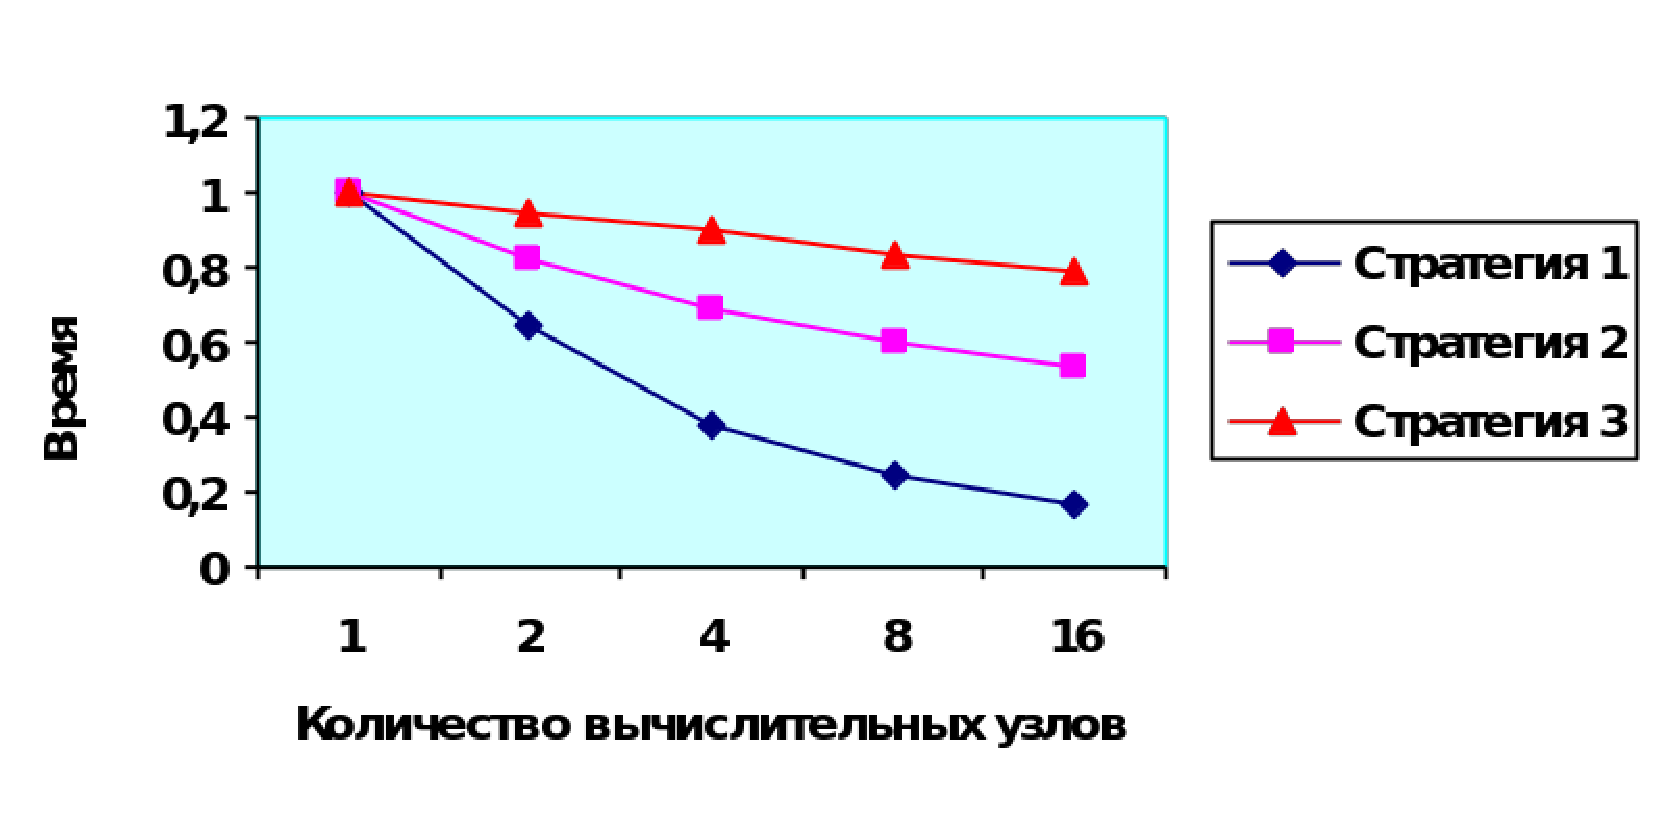
\includegraphics[width=0.6\linewidth]{pics/Parallel.eps}
	\caption{Результаты тестирования параллельной реализации алгоритмов АДТ, согласно представленной стратегии}
	\label{fig:parallel}
\end{figure}

Наибольшую эффективность, как и следовало ожидать, показала первая стратегия, естественно при наличии дизъюнктивного ветвления в исходной формуле. Под эффективностью понимается уменьшение затрачиваемого времени с увеличением количества вычислительных узлов.


%============================= РАВЕНСТВА =========================
\subsection{Равенства}
Для обработки предиката равенства, как правило, крайне неэффективно напрямую использовать аксиомы равенства (рефлексивность, симметричность, транзитивность, подстановочность) \app{без специальной адаптации алгоритмов АДТ}. Например, если формула содержит лишь один бинарный функциональный символ $f$ и один бинарный атомарный символ $A$, то в языке ПО--формул аксиомы равенства для такой формулы будут представлены следующим образом.
$$\left\lbrace
\begin{array}{l}
\forall x\colon\boldsymbol{True} - \exists\colon x = x \\
\forall x_1,y_1,x_2,_y2\colon x_1 = y_1, x_2 = y_2 - \exists\colon f(x_1,y_1) = f(x_2, y_2) \\
\forall x_1,y_1,x_2,_y2\colon x_1 = y_1, x_2 = y_2, A(x_1,y_1) - \exists\colon A(x_2,y_2)
\end{array}\right.
$$
Как видно, для каждого функционального и атомарного символа из формулы ставится в соответствие подформула-вопрос --- аксиома равенства. Явное использование таких аксиом, во--первых, усложняет структуру формулы (появляются лишние вопросы), во-вторых, \app{значительно} увеличивает число шагов вывода, в-третьих, генерирует много (потенциально бесконечно) фактов в базе, возможно не участвующих в выводе, а также мешающих выводу. Отметим, что данная проблема не так ужасна как в МР, поскольку в МР, в общем случае,  порождаются дополнительные дизъюнкты, а это соответствует порождению дополнительных вопросов в ПОФ. В исчислении ПО--формул порождаются лишь атомы-факты, за которыми проще \rem{наблюдать}{Вот надо подобрать четкий эквивалент.}, но тем не менее их много.

Очевидно, что вопросы-аксиомы равенства предназначены для того что бы выводить те и только те атомы-факты, которые эквивалентны по модулю $E(B)$, другим атомам-фактам из базы $B$. В данном случае $E(B)$ это все равенства из базы $B$.

Для того чтобы не использовать на прямую аксиомы равенства, предлагается генерировать эквивалентные по модулю $E(B)$ атомы-факты с помощью систем переписывания термов (СПТ) \cite{Nipkow}.

Для построения СПТ по равенствам в базе, используется известный алгоритм Кнута-Бендикса (Knuth-Bendix completion procedure) \cite{KBAlg}. Алгоритм Кнута-Бендикса, получая на входе множество атомов-равенств и редуцирующий порядок над термами \cite{Nipkow} строит эквивалентную конвергентную СПТ. Конвергентность СПТ означает что для каждого терма существует и только одна конечная форма (нормальная форма), которая может быть получена за конечное число переписываний. Под порядком над термами мы имеем ввиду отношение строгого частичного порядка над множеством термов. В нашем случае используется лексикографический порядок.

С помощью правил переписывания генерируются новые атомы-факты, эквивалентные, уже имеющимся в базе. В сочетании со стратегией удаления неиспользуемых фактов (стратегия экономии памяти), очевидно, что база не будет захламляться ненужными сгенерированными фактами.

Отметим, что такой подход не нарушает основных особенностей исчисления ПО--формул. Правило вывода сохраняется, остаётся единственным и унарным. Ответные подстановки по прежнему зависят лишь от базы, и не зависят от других вопросов. Базы попрежнему остаются независимы и содержат основные термы.

%В классическом подходе, в соответствии с определением ~\ref{ircond}, подстановка $\theta$ является ответом на вопрос, тогда и только тогда, когда $A \theta \subseteq B$ где $A$ --- конъюнкт вопроса, а $B$ --- конъюнкт базы. Поиск ответов есть задача поглощения, для решения которой, как правило, используется алгоритм матчинга \rem{, об этом уже писалось выше}{Это нужно?}. В случае ПО--формул используется основной матчинг, а в случае НЭЭ используется полуосновной матчинг. \rem{...}{Надо прокомментировать где-то ранее эти матчинги, или даже строго определить.}


%Для решения проблемы основного матчинга без явного использования аксиом равенства поставлена задача реализации основного матчинга с равенствами, которая формулируется следующим образом [microsoft]:
%\begin{quote}
%Для данного множества равенств $E(B)$, основного терма $t$ и терма $p$, который может содержать переменные, необходимо найти множество подстановок $\theta$, по модулю $E(B)$, такие что $E(B)\models t = p\theta$. Через $E(B)$ мы обозначим множество всех равенств в данной базе $B$. Две подстановки эквивалентны если их правые части попарно конгруэнты по модулю $E(B)$.
%\end{quote}

%С точки зрения реализации

%Для поиска таких ответов использован аппарат теории систем переписывания термов \cite{Nipkow}.

%=====================================================================
%==========================ХРАНИЛИЩЕ ОТВЕТОВ==========================
\subsection{Хранилище подстановок}
Хранилище подстановок предназначено для эффективной организации доступа алгоритмов к ответными подстановками и возможности организации механихзма бэктрэкинга, для приведения возможных ответов в предыдущие состояния (состояния на предыдущих шагах вывода).

Каждому атому конъюнкта вопроса соответствует чанк возможных подстановок, обеспечивающих матчинг этого атома с атомами из базы. Использование чанков связано с тем что необходимо точно определять на каком шаге какие подстановки были найдены. Для поиска ответа на вопрос, необходимо использовать алгоритм композиции подстановок для каждого атома из вопроса.

На рис.~\ref{fig:anbase} представлена схема хранения подстановок для каждого атома.

\begin{figure}[h]
	%\vspace{0.5cm}
	\centering
	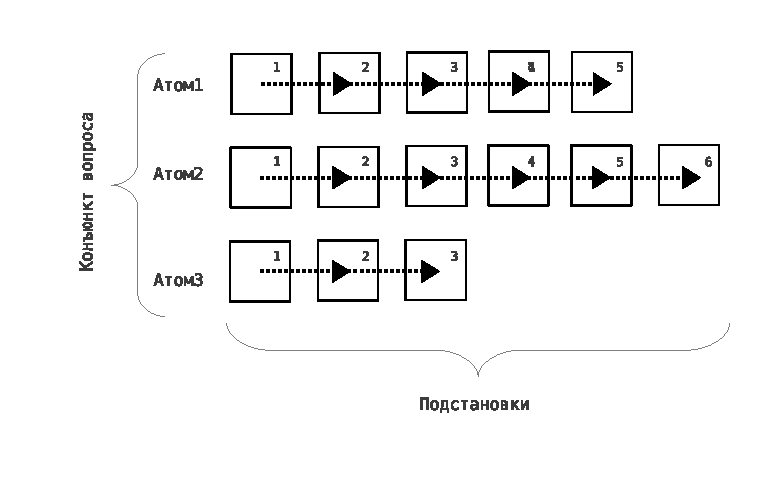
\includegraphics[width=0.6\linewidth]{pics/AnBase.eps}
	\caption{Подстановки}
	\label{fig:anbase}
\end{figure}

Из этой структуры выделяется ответ на вопрос, конъюнкту которого соответствует хранилище. Для этого комбинируются подстановки из каждого чанка по одной. При этом подстановки должны быть совместимы. Две подстановки совместимы если их левые части равны, а правые унифицируемы. Например, если есть подстановки $\{x \rightarrow a\}$ и $\{x \rightarrow b\}$, где $b$ есть константа, то эти подстановки несовместимы, поскольку $a$ и $b$ неунифицируемы. А подстановки $\{x \rightarrow f(a)\}$ и $\{x \rightarrow f(h)\}$, где $h$ есть НЭЭ, совместимы, поскольку $f(a)$ и $f(h)$ унифицируемы с подстановкой $\{h \rightarrow a\}$. Результатом комбинации будет объединение всех совместимых и унифицирующих подстановок.

Перебор подстановок из чанков производится \rem{последовательно}{Как декартово произведение? или еще как...}, это позволяет сохранить \rem{полноту}{Можно ли за счет состояния порождать др. состояние перебора, как у меня было. Или обязательно все подстановки хранить.}.

%=================================================================================
%==================================СТАНДАРТНАЯ СТРАТЕГИЯ==========================
%=================================================================================
\subsection{Стандартная стратегия \app{поиска логического вывода}}
Главное свойство стандартной стратегии \app{поиска логического вывода} заключается в её полноте. Для полноты вывода необходимо организовать полный последовательный перебор всевозможных ответов на все вопросы. Для этого используются возможности дерева состояний вывода и хранилища ответов. \rem{...}{Надо, я так понял, стратегию описать здесь подробно. Или зачем тогда раздел?}


%%% Local Variables:
%%% mode: latex
%%% TeX-master: "dis"
%%% End:
